% Options for packages loaded elsewhere
\PassOptionsToPackage{unicode}{hyperref}
\PassOptionsToPackage{hyphens}{url}
%
\documentclass[
  11pt,
  a4paper]{article}
\usepackage{amsmath,amssymb}
\usepackage{iftex}
\ifPDFTeX
  \usepackage[T1]{fontenc}
  \usepackage[utf8]{inputenc}
  \usepackage{textcomp} % provide euro and other symbols
\else % if luatex or xetex
  \usepackage{unicode-math} % this also loads fontspec
  \defaultfontfeatures{Scale=MatchLowercase}
  \defaultfontfeatures[\rmfamily]{Ligatures=TeX,Scale=1}
\fi
\usepackage{lmodern}
\ifPDFTeX\else
  % xetex/luatex font selection
\fi
% Use upquote if available, for straight quotes in verbatim environments
\IfFileExists{upquote.sty}{\usepackage{upquote}}{}
\IfFileExists{microtype.sty}{% use microtype if available
  \usepackage[]{microtype}
  \UseMicrotypeSet[protrusion]{basicmath} % disable protrusion for tt fonts
}{}
\makeatletter
\@ifundefined{KOMAClassName}{% if non-KOMA class
  \IfFileExists{parskip.sty}{%
    \usepackage{parskip}
  }{% else
    \setlength{\parindent}{0pt}
    \setlength{\parskip}{6pt plus 2pt minus 1pt}}
}{% if KOMA class
  \KOMAoptions{parskip=half}}
\makeatother
\usepackage{xcolor}
\usepackage[a4paper, margin=1in]{geometry}
\usepackage{graphicx}
\makeatletter
\def\maxwidth{\ifdim\Gin@nat@width>\linewidth\linewidth\else\Gin@nat@width\fi}
\def\maxheight{\ifdim\Gin@nat@height>\textheight\textheight\else\Gin@nat@height\fi}
\makeatother
% Scale images if necessary, so that they will not overflow the page
% margins by default, and it is still possible to overwrite the defaults
% using explicit options in \includegraphics[width, height, ...]{}
\setkeys{Gin}{width=\maxwidth,height=\maxheight,keepaspectratio}
% Set default figure placement to htbp
\makeatletter
\def\fps@figure{htbp}
\makeatother
\setlength{\emergencystretch}{3em} % prevent overfull lines
\providecommand{\tightlist}{%
  \setlength{\itemsep}{0pt}\setlength{\parskip}{0pt}}
\setcounter{secnumdepth}{-\maxdimen} % remove section numbering
\ifLuaTeX
\usepackage[bidi=basic]{babel}
\else
\usepackage[bidi=default]{babel}
\fi
\babelprovide[main,import]{spanish}
% get rid of language-specific shorthands (see #6817):
\let\LanguageShortHands\languageshorthands
\def\languageshorthands#1{}
\usepackage{amsmath}
\usepackage{amsfonts}
\usepackage{amssymb}
\usepackage{booktabs}
\usepackage{float}
\usepackage{caption}
\captionsetup[figure]{labelsep=period, font=small}
\captionsetup[table]{labelsep=period, font=small}
\ifLuaTeX
  \usepackage{selnolig}  % disable illegal ligatures
\fi
\IfFileExists{bookmark.sty}{\usepackage{bookmark}}{\usepackage{hyperref}}
\IfFileExists{xurl.sty}{\usepackage{xurl}}{} % add URL line breaks if available
\urlstyle{same}
\hypersetup{
  pdftitle={Reporte Ejecutivo: Análisis Bootstrap y Monte Carlo para la Estimación de \$ au( heta) = P(X=0)\$ en una Distribución Poisson},
  pdfauthor={Omar Flores (Basado en el script R proporcionado)},
  pdflang={es},
  hidelinks,
  pdfcreator={LaTeX via pandoc}}

\title{Reporte Ejecutivo: Análisis Bootstrap y Monte Carlo para la
Estimación de \$ au( heta) = P(X=0)\$ en una Distribución Poisson}
\author{Omar Flores (Basado en el script R proporcionado)}
\date{21 de May de 2025}

\begin{document}
\maketitle
\begin{abstract}
Este reporte presenta los resultados de análisis estadísticos realizados
para estimar el parámetro \(\tau(\theta) = e^{-\theta} = P(X=0)\) de una
distribución Poisson, utilizando el estimador UMVUE
\(\hat{\tau} = \left(\frac{n-1}{n}\right)^{\sum X_i}\). Se aplicaron
métodos de Monte Carlo y bootstrap no paramétrico según lo especificado,
y se evaluó el desempeño de los intervalos de confianza bootstrap. Todos
los análisis se implementaron en R, utilizando \texttt{set.seed(1234)}
para reproducibilidad. Las cifras y tablas aquí presentadas se derivan
de la ejecución de dicho script.
\end{abstract}

\hrulefill

\hrulefill
\vspace{1em}

\section{Introducción}

El objetivo principal es la estimación del parámetro
\(\tau(\theta) = e^{-\theta}\), que representa la probabilidad de
observar un cero en una variable aleatoria \(X\) que sigue una
distribución de Poisson con parámetro \(\theta\). El estimador utilizado
es \(\hat{\tau} = \left(\frac{n-1}{n}\right)^{\sum_{i=1}^n X_i}\), el
cual se indica es el estimador insesgado de mínima varianza uniforme
(UMVUE) de \(\tau(\theta)\).

Este reporte se divide en tres partes principales:

\begin{enumerate}
    \item \textbf{Simulación Monte Carlo (MC):} Aproximación del valor esperado $E(\hat{\tau})$ y la varianza $V(\hat{\tau})$ cuando $\theta$ es conocido.
    \item \textbf{Bootstrap No Paramétrico:} Estimación de $\tau(\theta)$, $V(\hat{\tau})$ y construcción de un intervalo de confianza para $\tau(\theta)$ a partir de una muestra observada específica, sin asumir conocimiento de $\theta$.
    \item \textbf{Estudio de Simulación de Cobertura:} Evaluación de la probabilidad de cobertura de los intervalos de confianza bootstrap no paramétricos.
\end{enumerate}

Para todos los análisis inferenciales no especificados, se utiliza un
nivel de significancia \(\alpha = 0.05\).

\section{Parte a: Simulación Monte Carlo (Distribución Conocida)}

En esta sección, se utiliza el método Monte Carlo para aproximar el
valor esperado y la varianza del estimador \(\hat{\tau}\). Se asume que
los datos provienen de una distribución Poisson(\(\theta\)) con
\(\theta = 1.3\), y se generan muestras de tamaño \(n=20\). Se
realizaron \(B = 10,000\) réplicas Monte Carlo.

\subsection{Metodología}

Para cada una de las \(B=10,000\) réplicas:

\begin{enumerate}
    \item Se generó una muestra aleatoria $X_1, \dots, X_{20}$ de una distribución Poisson($\theta=1.3$).
    \item Se calculó $\hat{\tau}_b = \left(\frac{20-1}{20}\right)^{\sum X_i}$ para la muestra $b$.
\end{enumerate}

Luego, \(E(\hat{\tau})\) se aproximó por
\(\frac{1}{B}\sum_{b=1}^B \hat{\tau}_b\) y \(V(\hat{\tau})\) por
\(\frac{1}{B-1}\sum_{b=1}^B (\hat{\tau}_b - \bar{\hat{\tau}})^2\).

\subsection{Resultados}

El valor verdadero de \(\tau(\theta)\) para \(\theta=1.3\) es
\(\tau(1.3) = e^{-1.3}\). Los resultados obtenidos de la simulación
Monte Carlo se resumen en la Tabla \ref{tab:mc_results}.

\begin{table}[H]
    \centering
    \caption{Resultados de la Simulación Monte Carlo para $\hat{\tau}$ ($\theta=1.3$, $n=20$, $B=10,000$)}
    \label{tab:mc_results}
    \begin{tabular}{lc}
        \toprule
        Métrica & Valor \\
        \midrule
        Valor verdadero $\tau(1.3) = e^{-1.3}$ & 0.27253 \\
        Estimación MC de $E(\hat{\tau})$ & 0.27210 \\
        Estimación MC de $V(\hat{\tau})$ & 0.0050471 \\
        \bottomrule
    \end{tabular}
\end{table}

El histograma de las \(10,000\) estimaciones \(\hat{\tau}_b\) obtenidas
se muestra en la Figura @ref(fig:hist-mc-a).

\begin{figure}

{\centering 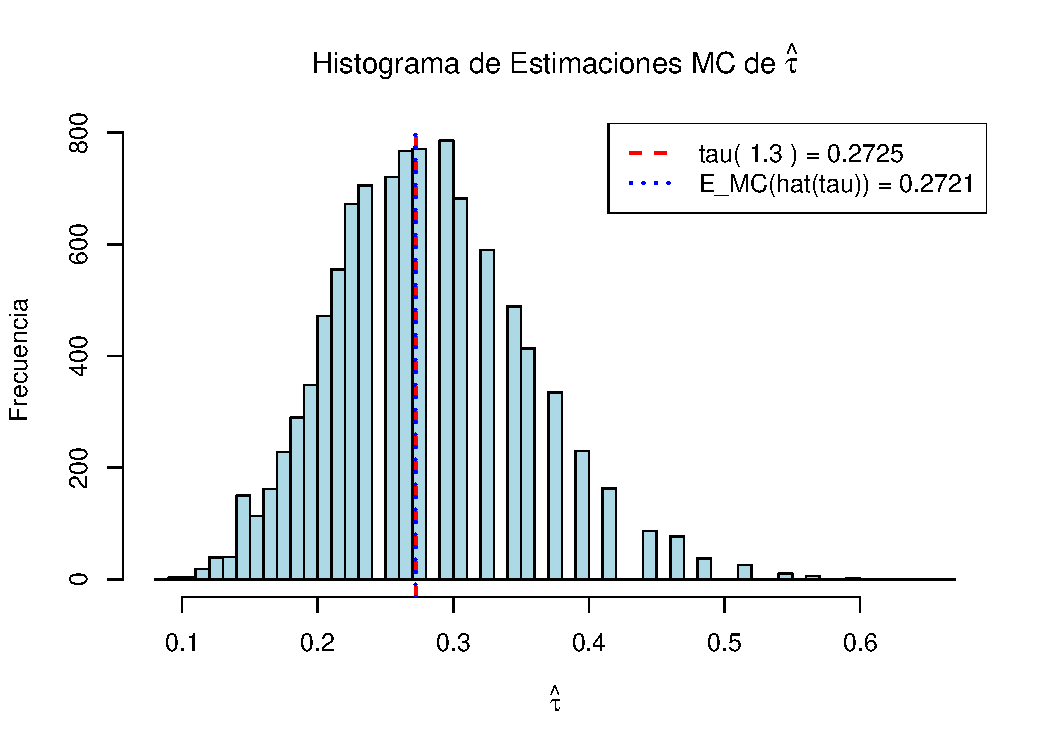
\includegraphics{/app/Tarea2/Tarea2_1_files/figure-latex/hist-mc-a-1} 

}

\caption{Histograma de las estimaciones $\hat{\tau}$ obtenidas mediante simulación Monte Carlo. La línea roja discontinua indica el valor verdadero $\tau(1.3)$ y la línea azul punteada indica la media de las estimaciones MC.}\label{fig:hist-mc-a}
\end{figure}

\section{Parte b: Bootstrap No Paramétrico (Muestra Observada)}

En esta sección, se utiliza el método bootstrap no paramétrico para
analizar el estimador \(\hat{\tau}\) a partir de una única muestra
observada, sin suponer conocimiento previo de \(\theta\) o la forma
exacta de la distribución (aunque el estimador \(\hat{\tau}\) se deriva
bajo el supuesto Poisson).

\subsection{Datos y Metodología}

La muestra observada es
\(X = (1, 2, 0, 0, 1, 1, 0, 1, 0, 0, 1, 1, 0, 1, 1, 0, 0, 1, 1, 0)\),
con \(n=20\). Se generaron \(B=10,000\) muestras bootstrap:

\begin{enumerate}
    \item Se calculó $\hat{\tau}_{obs}$ a partir de la muestra original.
    \item Para cada una de las $B=10,000$ réplicas bootstrap:
    \begin{enumerate}
        \item Se generó una muestra bootstrap $X_1^*, \dots, X_{20}^*$ muestreando con reemplazo de la muestra observada $X$.
        \item Se calculó $\hat{\tau}_b^*$ para la muestra bootstrap $b$.
    \end{enumerate}
    \item La varianza de $\hat{\tau}$ se estimó como la varianza de las $\hat{\tau}_b^*$.
    \item Se construyó un intervalo de confianza (IC) del 95\% para $\tau(\theta)$ utilizando el método de los percentiles sobre las $\hat{\tau}_b^*$.
\end{enumerate}

\subsection{Resultados}

Los resultados del análisis bootstrap no paramétrico se resumen en la
Tabla \ref{tab:boot_results_b}.

\begin{table}[H]
    \centering
    \caption{Resultados del Bootstrap No Paramétrico para $\hat{\tau}$ (Muestra observada, $n=20$, $B=10,000$)}
    \label{tab:boot_results_b}
    \begin{tabular}{lc}
        \toprule
        Métrica & Valor \\
        \midrule
        Estimación $\hat{\tau}_{obs}$ (de la muestra original) & 0.54036 \\
        Estimación Bootstrap de $V(\hat{\tau})$ & 0.0053082 \\
        IC del 95\% para $\tau(\theta)$ (percentiles) & (0.41812, 0.69834) \\
        \bottomrule
    \end{tabular}
\end{table}

El histograma de las \(10,000\) estimaciones bootstrap
\(\hat{\tau}_b^*\) se muestra en la Figura @ref(fig:hist-bootstrap-b).

\begin{figure}

{\centering 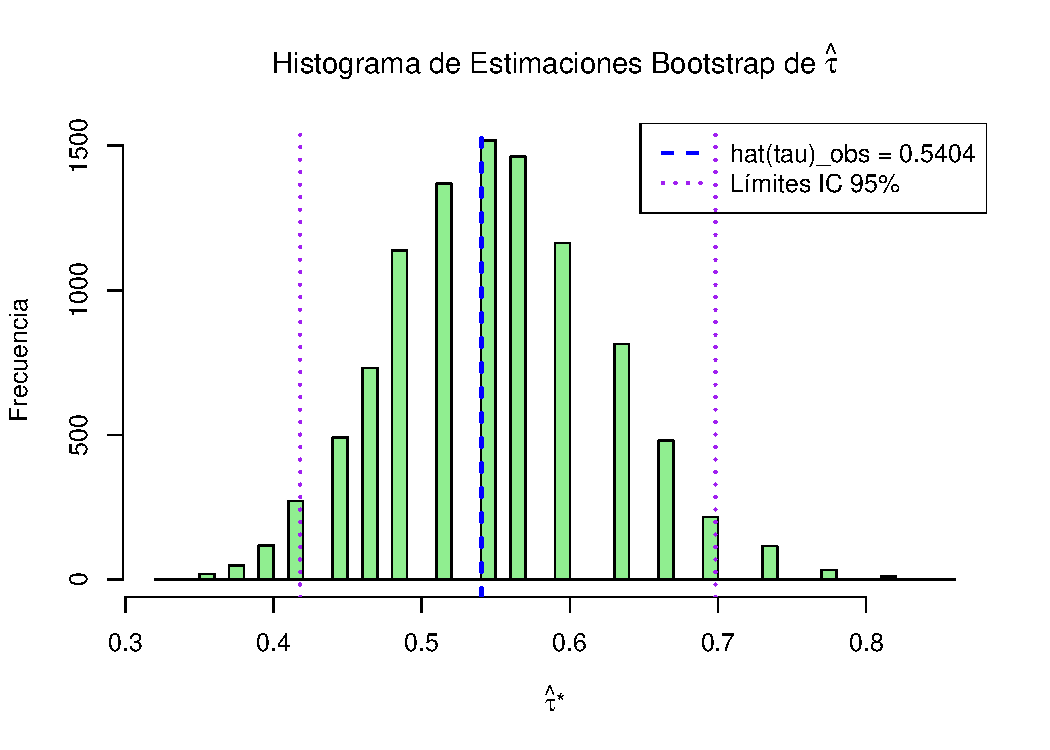
\includegraphics{/app/Tarea2/Tarea2_1_files/figure-latex/hist-bootstrap-b-1} 

}

\caption{Histograma de las estimaciones bootstrap $\hat{\tau}^*$. La línea azul discontinua indica $\hat{\tau}_{obs}$ y las líneas púrpuras punteadas los límites del IC del 95\%.}\label{fig:hist-bootstrap-b}
\end{figure}

Comentario sobre los resultados si la muestra proviniera de
Poisson(\(\theta=1.3\)): El valor verdadero
\(\tau(1.3) = e^{-1.3} \approx 0.27253\). La estimación observada
\(\hat{\tau}_{obs} = 0.54036\). El IC Bootstrap {[}0.41812, 0.69834{]}
\textbf{no contiene} el valor \(\tau(1.3)\).

\section{Parte c: Estudio de Simulación para Cobertura del IC Bootstrap}

Se realizó un estudio de simulación para evaluar el desempeño
(probabilidad de cobertura) de los intervalos de confianza del 95\%
obtenidos mediante el método bootstrap no paramétrico (percentiles) para
\(\hat{\tau}\).

\subsection{Metodología}

Se repitió el siguiente procedimiento \(M=1,000\) veces:

\begin{enumerate}
    \item Se generó una muestra aleatoria de tamaño $n=20$ de una distribución Poisson($\theta=1.3$). El verdadero valor del parámetro de interés es $\tau(1.3) = e^{-1.3}$.
    \item Con esta muestra generada, se construyó un intervalo de confianza del 95\% para $\tau(\theta)$ usando el método bootstrap no paramétrico con $B=10,000$ réplicas (como en la Parte b).
    \item Se verificó si el intervalo de confianza resultante contenía el valor verdadero $\tau(1.3)$.
\end{enumerate}

La probabilidad de cobertura se estimó como la proporción de los \(M\)
intervalos que contenían el valor verdadero.

\subsection{Resultados}

Los resultados del estudio de simulación de cobertura se presentan en la
Tabla \ref{tab:coverage_results_c}.

\begin{table}[H]
    \centering
    \caption{Resultados del Estudio de Simulación de Cobertura del IC Bootstrap ($M=1,000$ sims, $\theta=1.3$, $n=20$, $B=10,000$ por IC)}
    \label{tab:coverage_results_c}
    \begin{tabular}{lc}
        \toprule
        Métrica & Valor \\
        \midrule
        Nivel de Confianza Nominal & 0.95 \\
        Probabilidad de Cobertura Observada & 0.9340 \\
        Número de ICs que cubrieron $\tau(1.3)$ (de $M=1,000$) & 934 \\
        $p$-valor (Prueba Binomial $H_0$: Cobertura = 0.95) & 0.0242 \\
        \bottomrule
    \end{tabular}
\end{table}

Conclusión de la prueba binomial: Se rechaza H0. La cobertura observada
(0.934) difiere significativamente de la nominal (0.95) al nivel alpha =
0.05.

\vspace{2em}
\hrulefill

```

\end{document}
